\chapter{Images Segmentation}
\label{ch:image_segmentation}
Within this chapter I will introduce both classical and modern segmentation methods as well as competitive mathematical background behind them.

Initially, the notion of segmentation within image analysis stands for the process of classifying pixels into groups which corresponds to the same type or class. The segmentation allows to obtain more meaningful and potentially hidden information from original images, what let to bring indeed numerous insights for various business problems. For instance, in medicine analysis segmentation has many uses cases like a measure volume of an organ, render a 3D view of an organ, surface-based registration and many others. Before moving forward I will explicitly distinguish segmentation types from general point of view.

Segmentation can be broadly divided into two types. Assume following Figure \ref{fig:image_segmentation} below. 
\begin{figure}[h]
    \centering
    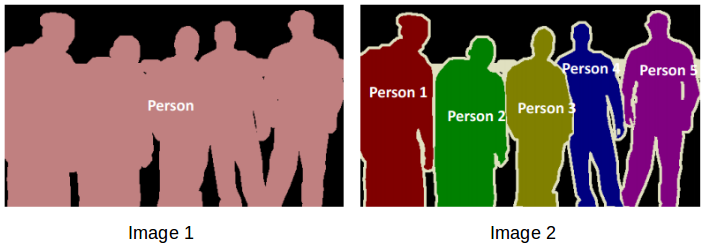
\includegraphics[width=9cm]{images/segmentation_types.png}
    \caption{Image 1: is an example of semantic segmentation. Image 2 is an example of instance segmentation.}
    \label{fig:image_segmentation}
\end{figure}

On the left side image, every pixel belongs to a particular class (either background or person). Also, all the pixels belonging to a particular class are represented by the same color (background as black and person as pink). This type of segmentation is called "semantic segmentation".  

On the right hand image we also has assigned a particular class to each pixel of the image. However, different objects of the same class have different colors (Person 1 as red, Person 2 as green, background as black, etc.). This type of segmentation is called "instance segmentation".

\section{Classical Segmentation Methods} 
Now we are good to go with classical segmentation methods section. I will cover basic thresholding method, then modified version of thresholding so called region growing. Afterwards I will speak about edge detection segmentation and clustering based segmentation. On top of that I will demonstrate the performance of each dedicated technique within the following baseline Figure \ref{fig:sample_vertebrae} of vertebrae.

\begin{figure}[h]
    \centering
    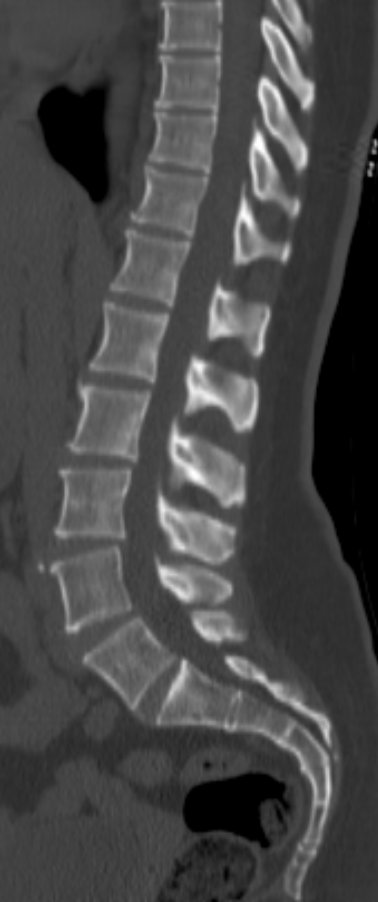
\includegraphics[width=2cm]{images/sample_vertebrae.jpeg}
    \caption{Sample CT scan of vertebrae.}
    \label{fig:sample_vertebrae}
\end{figure}


\subsection{Region Based Segmentation}
Sometimes region based segmentation method can be named as thresholding. It is the simplest method for classifying pixels based on solely on their intensity values. In thresholding we have options to choose either upper and lower bound and select pixels in predefined range or to choose just one threshold value which can be for instance the mean of the original image values. 

Mathematically, the algorithm can be defined as:
\[
    f(x, y)= 
\begin{cases}
    0   ,& \text{if } f(x, y) > T \\
    255 ,& \text{otherwise}
\end{cases}
\]

After applying the algorithm with the mean threshold on the baseline Figure \ref{fig:sample_vertebrae}, I had obtained following resulting segmented image:

\begin{figure}[h]
    \centering
    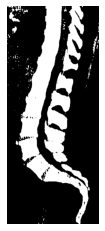
\includegraphics[width=2cm]{images/sample_vertebrae_thresholding.png}
    \caption{Applied thresholding algorithm for sample CT scan of vertebrae.}
    \label{fig:sample_vertebrae}
\end{figure}

The problem within simple thresholding is that it does not take into consideration any spatial information, meaning each pixel is evaluated no matter where it is located as well as each time we have to find best way to define the either threshold value or range of values.    


\subsection{Region Growing Segmentation}
Unlike basic thresholding, region growing -- which is iterative method -- starts with the small set of seed pixels and grow out from them.

The method functionality can be easily represented within any basic draw editor. To do that we will draw empty grid rectangle and afterwards select interested regions and apply function named 'flat fill' with chosen color. As a result it can be noticed the naive functionality handled the problem of tricking-out the selected regions by chosen color. This is so called region growing thresholding.    

\begin{figure}[h]
    \centering
    \begin{minipage}[b]{0.4\textwidth}
    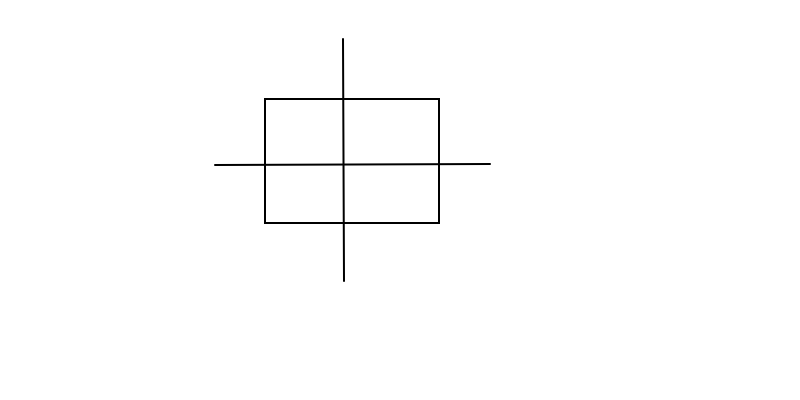
\includegraphics[width=\textwidth]{images/grow_region_0.png}
    \caption{Empty grid rectangle.}
    \end{minipage}
    \hfill
    \begin{minipage}[b]{0.4\textwidth}
    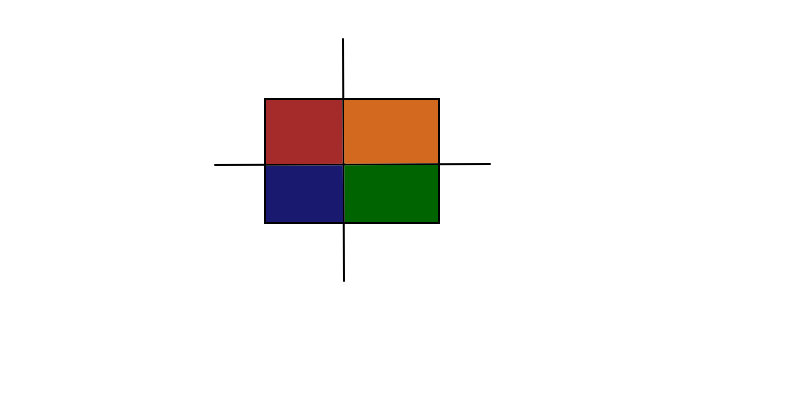
\includegraphics[width=\textwidth]{images/grow_region_1.png}
    \caption{Filled grid rectangle.}
    \end{minipage}
\end{figure}

Now, let us see how it is done from code base perspective.
\begin{lstlisting}
do
  for each pixel in the set
    for each of it's neighbours not in the set
      if the intensity falls between the thresholds
        add it to the set
      endif
    next neighbour
  next pixel
until no pixel were added in the last pass   
\end{lstlisting}

\newcolumntype{C}[1]{>{\centering\let\newline\\\arraybackslash\hspace{0pt}}m{#1}}
\newcolumntype{L}[1]{>{\raggedright\let\newline\\\arraybackslash\hspace{0pt}}m{#1}}

Example: There is set of pixels $4 \cdot 4$ which should be colored. The cells which denoted by red color is already tricking-out. The task is fill rest with red color based on defined thresholding range.       

\begin{tabular}{C{7cm}  L{7cm}}
    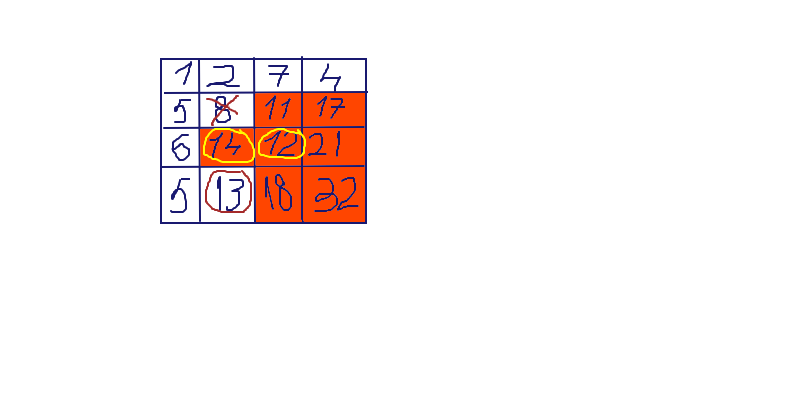
\includegraphics[width=12cm]{images/grow_region_3.png} & Thresholds: include a pixel if $10 \leq intensity \leq 100$ \newline 
    \begin{lstlisting}
    Looking at 14 ...
    up: 8 -> exclude (not in range)
    right: 12 -> skip (already in the set)
    down: 13 -> include as a new entry
    left: 6 -> exclude (not in range)
    \end{lstlisting}
\end{tabular}

Exactly the same way growing region thresholding method may be applied for medical images of different image modalities.
\begin{figure}[h]
    \centering 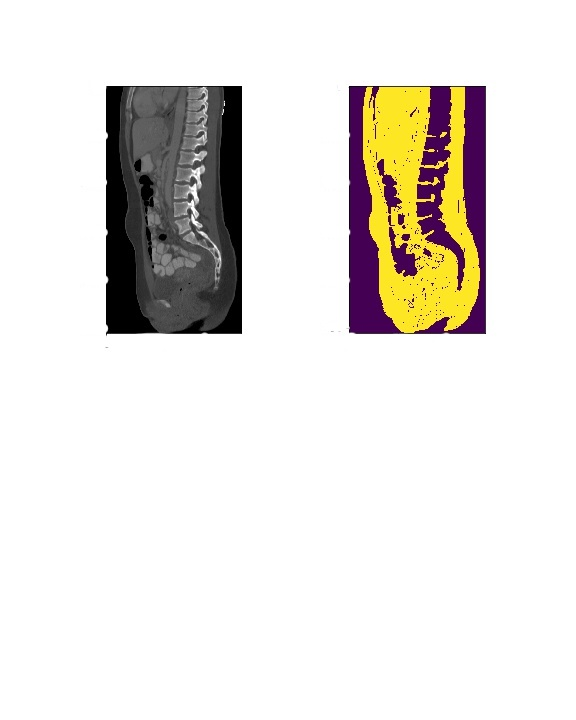
\includegraphics[width=8cm]{images/ct-spine-grow-region-segmented.jpg}
    \vspace*{-50mm} \caption {Original CT spine versus Grow Region thresholding Segmented CT spine.}
\end{figure}    

There is a huge potential room for improvements making the method more sophisticated by coming up with different conditions for inclusion/exclusion of pixels.

\subsection{k-Means Clustering}
k-Means algorithm is very simple clustering method whereas usually the data set is represented as the a scatter plot in some feature space.

For instance, a pixel could be represented by 3 dimensional feature space, where feature space is defined by retrieving from the image following pixel-wise features:
\begin{enumerate}
    \setlength\itemsep{0.05em}
    \item Intensity
    \item Gradient magnitude
    \item Laplacian
\end{enumerate}

First let us clarify the target results we are looking for by considering the very trivial task.
Assume, there is colorful triangle which should be clustered and represented in some feature space. Afterwards we can clearly see 3 different colors which denotes 3 clusters/groups.

\begin{figure}[h]
    \centering
    \begin{minipage}[b]{0.4\textwidth}
    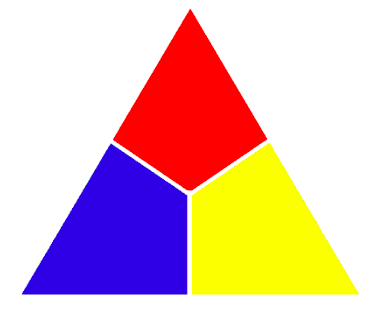
\includegraphics[width=\textwidth]{images/k_mean_triangle.png}
    \caption{Colorful triangle.}
    \end{minipage}
    \hfill
    \begin{minipage}[b]{0.4\textwidth}
    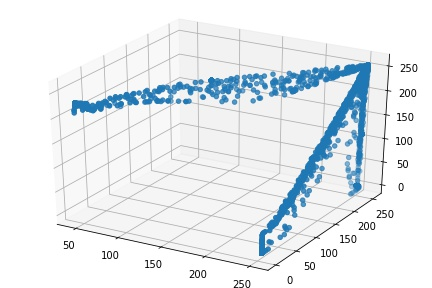
\includegraphics[width=\textwidth]{images/k_mean_triangle_clustered.jpg}
    \caption{Feature space representation.}
    \end{minipage}
\end{figure}


As for now, imagine, the user specified k the number of clusters, meaning how many different tissue types are in the image.
Hence, the algorithm may be defined as:
\begin{lstlisting}
1. (randomly) choose k regressors as prototype
2. assign each scatter point ('feature vector') to it's nearest regressor
3. recalculate new prototypes (the mean of it's members)
4. if the prototypes changed significantly -> go to the step 2 
\end{lstlisting}
To demonstrate the method we are going to proceed with the same CT spine scan data which had used for region growing thresholding. As for regressors number (clusters number) we will choose $k=3$.  

Eventually, as results show, clustering is a really efficient way for image segmentation, because of both intensity of scatter plot (feature space) and different representations of clusters.

\begin{figure}[h]
    \centering 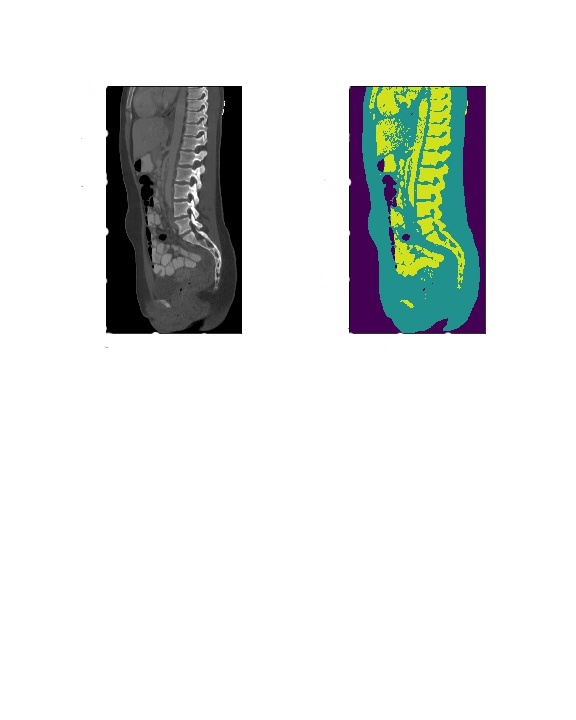
\includegraphics[width=8cm]{images/ct-spine-k-means-segmented.jpg}
    \vspace*{-50mm} \caption {Original CT spine versus k-Means Segmented CT spine.}
\end{figure}


\section{Modern Segmentation Methods}
\section{Neuron}
Typically, neurons are kind of information messengers who make use of electrical and chemical gusts to transfer information across all brain moreover between brain and rest of the nervous system.

\subsection{Biological neuron}
A neuron is a component that makes up the entire human nervous system. Almost all neurons are structured roughly the same. So, a neuron has a neuron nucleus, which is also called the neuron body. An electrical charge is accumulated in the body of a neuron. From the body of the neuron there are many processes: there are small processes and large processes. The little outgrowths are so called dendrites. Through these processes, a signal from other neurons comes to our neuron. There is a large scion. This process is called an axon. A neuron transmits a signal to other neurons along the axon. The place where the axon of another neuron connects to the dendrites of our neuron is called a 'synapse'. The synapse is where the dendrite and axon meet. A synapse can be strong or it can be weak. If the synapse is strong, then the signal that is transmitted along the axon of the neuron will almost completely go to our neuron. If the synapse is weak, then practically no charge will cross from the axon of another neuron to our neuron. The synapse can change over time. Depending on the circumstances, the synapse can get stronger or it can get weaker. It is with the synapse tuning that the training of the biological neural network and, accordingly, the human nervous system is connected.

Considered visualization of the described above processes is as follows:
\begin{figure}[h]
    \centering 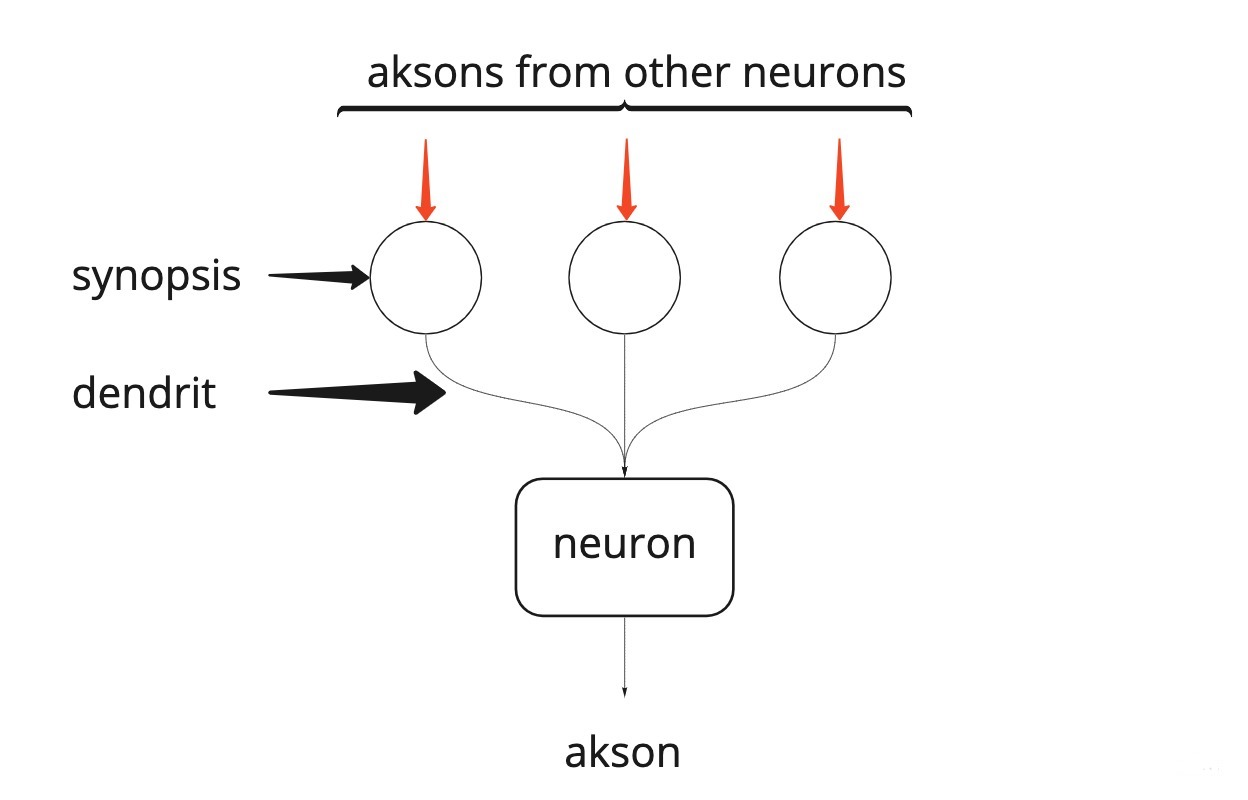
\includegraphics[width=8cm]{images/biological_neuron.jpg}
    \caption {Biological model of neuron.}
\end{figure}    

\subsection{Mathematical model of neuron}
Initially for simplicity we will represent neuron mathematical model graphically. It should be taken into consideration, the red characters denote tune parameters of the neuron.     
\begin{figure}[h]
    \centering 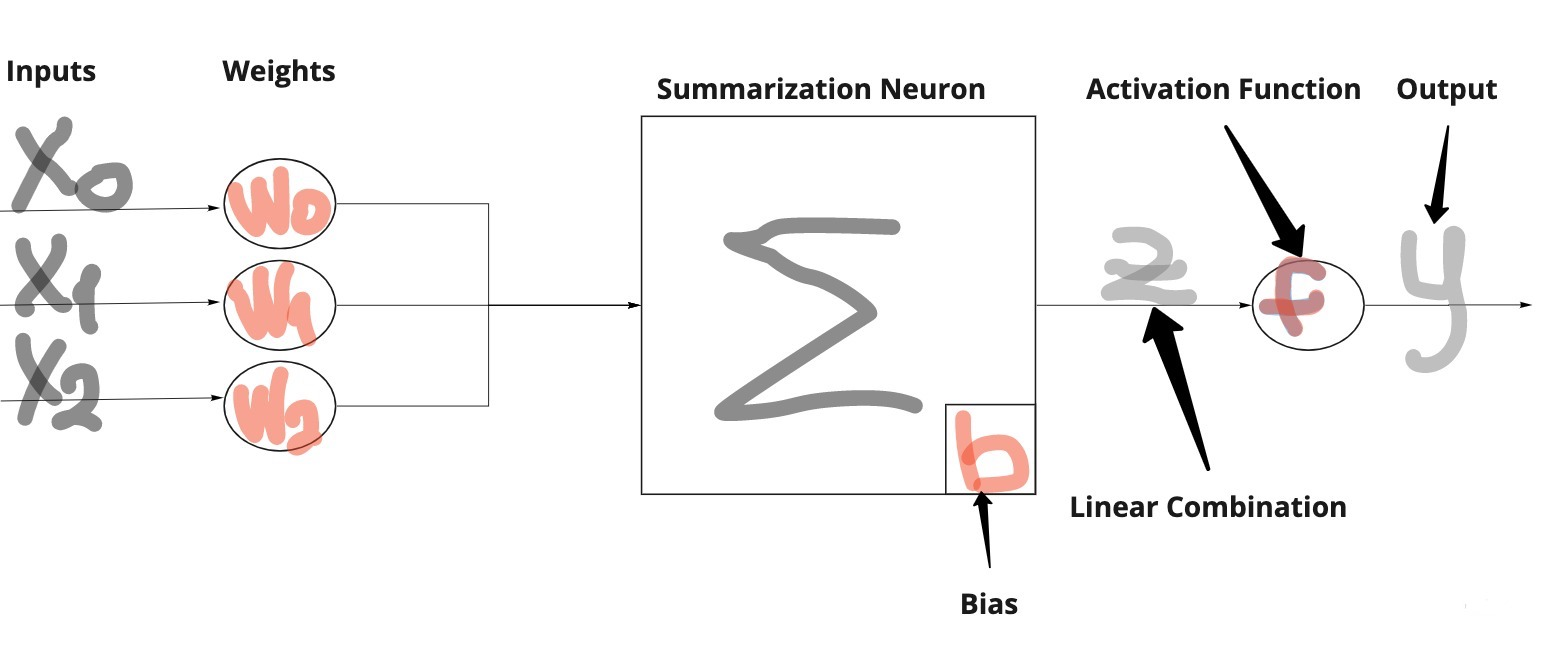
\includegraphics[width=8cm]{images/neuron_math_model.jpg}
    \caption {Mathematical model of neuron.}
\end{figure} 

In the mathematical model of the neuron, the body of the neuron, where the input signals accumulates, is denoted by a summarizing neuron. In addition, the biological neuron also has axons and dendrites, which get the inputs and send the outputs. Accordingly, in our mathematical model of the neuron, we will add inputs and outputs to the summarizing neuron. It's also worth keep in mind the biological neuron applies some actions with the signals that come into it, namely, it accumulates charge until it reaches some point and only after that forwards it further. This is what we will do in the mathematical model of the neuron using the activation functions.

Afterwards, let us mathematically define model of neuron as:
\begin{align*}
y = f(z) = f(w_0 \cdot x_0+w_1 \cdot x_1+w_2 \cdot x_2+b) = f(\sum\limits_{i=0}^{N-1} w_i \cdot x_i+b) = f(\langle w, x \rangle + b)
\end{align*}
Where: $x_0, x_1, x_2$: inputs, $w_0, w_1, w_2$: weights,  $b$: some bias for increasing non-linearity, $f(z)$: some activation function. 

Inputs can be either single number or vector of numbers. As for weights, we mainly should remember they are tuned parameters. Moreover it should be considered 2 potential situations to manage with. The first one is initialization of the weights. Here we have multiple options whereas we literally can define them either randomly or apply special initialisation techniques such as 'He' initialization or 'Xavier' initialization and others. The second situation we should be aware of is to somehow change the weights during model fitting, meaning weights should be changed in iterative manner from epoch to epoch. To do this we will apply backpropagation algorithm. Concerning the bias, which is like a weights, meaning tuned parameter, we can consider it allows to shift the activation function by adding a constant to the input of neuron. Hence, the last but not least component is activation function. In simplified terms, activation function is used to determine the output of neuron in a manner: 'yes' or 'no'. It maps the resulting values in range between 0 to 1 or -1 to 1.            

\section{Activation function}
There is a significant number of various activation functions. Let us assume the very basic one named 'step function' and figure out from general point of view how it works in both mathematical and geometrical sense.   
The 'step function' defined as:
\begin{align*}
f(x) = \begin{cases} 0, & \mbox{if } x\mbox{ $\leq$ 0} \\ 1, & \mbox{if } x\mbox{ $>$ 0} \end{cases}
\end{align*}

The function has 2 strongly distinguished values: '0' and '1'. The 'spot' where the function changes it's value from '0' to '1' is named as dividing surface. Hence, the dividing surface 'spot' is where the argument of activation function is equal '0'.

\begin{figure}[h]
    \centering 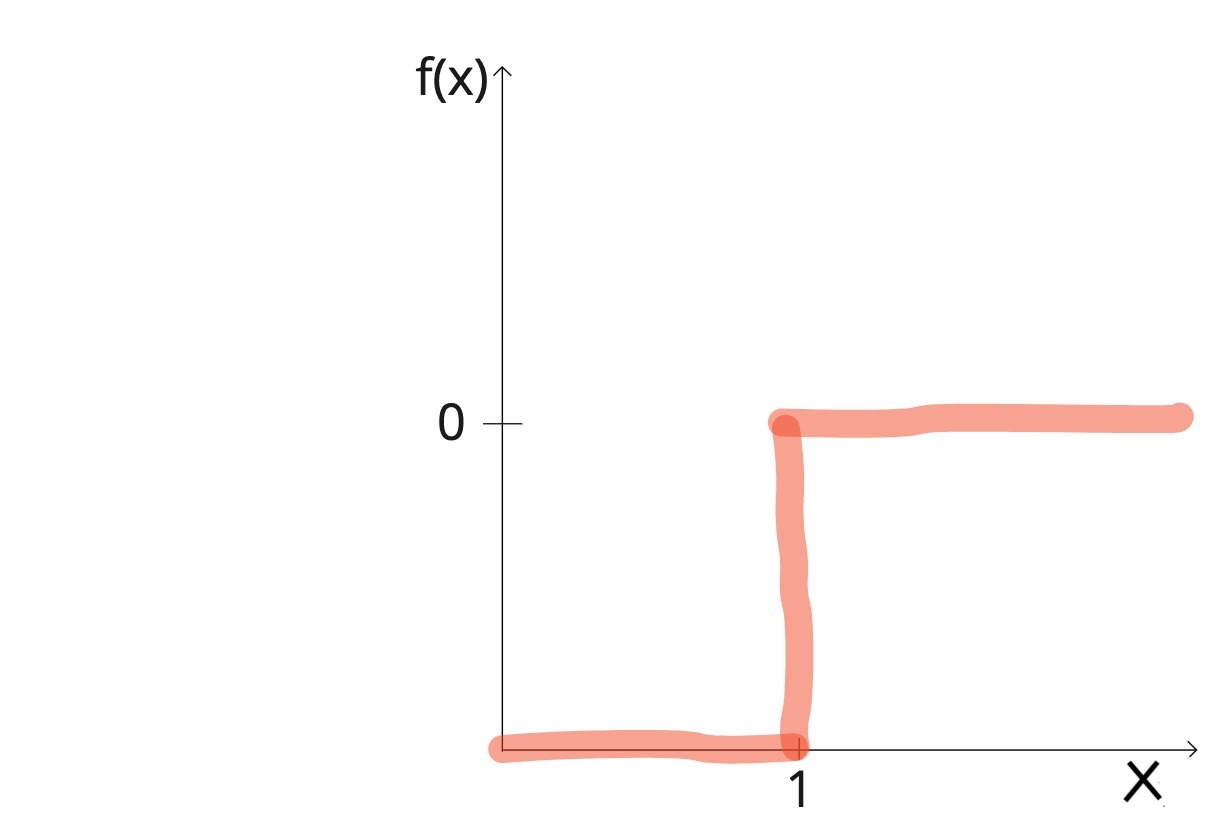
\includegraphics[width=8cm]{images/step_function.jpg}
    \caption {Geometrical representation of step function.}
\end{figure}

The geometrical representation of step function can be derived as following. Assume there is the neuron formula:
\begin{align*}
y = f(\langle w, x \rangle + b)
\end{align*}

The neuron does some linear operation, which is denoted by 2 parameters: $w$ (vector of weights) and $b$ (bias). Accordingly, the dividing surface is defined by following equitation which denotes equitation of straight line:
\begin{align*}
\langle w, x \rangle + b = 0
\end{align*}

\begin{figure}[h]
    \centering 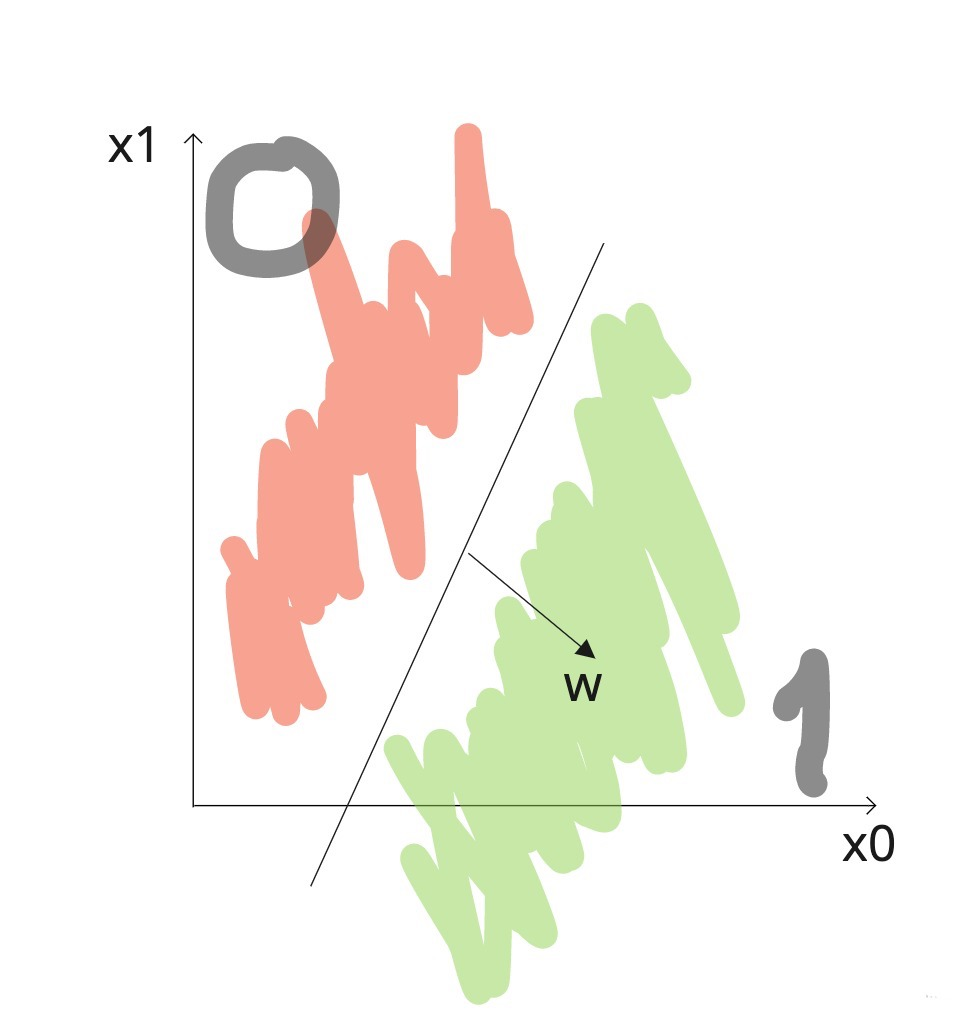
\includegraphics[width=8cm]{images/dividing_surface.jpg}
    \caption {Sample geometrical representation of dividing surface for single neuron.}
\end{figure}

From the one side the value of step function is equal '1' and from the other '0'. The activation function is equal '1' that side of dividing surface where the vector 'w' points out.

As it was mentioned earlier, step function is not the only one activation function. There is for instance 'sigmoid' activation function which unlike step function does not have discontinuity point at zero. 

The sigmoid activation function formed as:
\begin{align*}
\sigma(x) = \dfrac{1}{1+e^x}
\end{align*}

\[ \sigma(x) = \begin{cases} 1, & \mbox{if } x\mbox{$\xrightarrow{} + \infty$} \\ 0, & \mbox{if } x\mbox{$\xrightarrow{} - \infty$} \end{cases} \]

The rectified linear activation function for short is a piece-wise linear function which outputs input directly if it is positive otherwise outputs zero. It has become the default activation function for many types of neural networks because a model that uses it is easier to train and often achieves better performance.

\begin{figure}[h]
    \centering 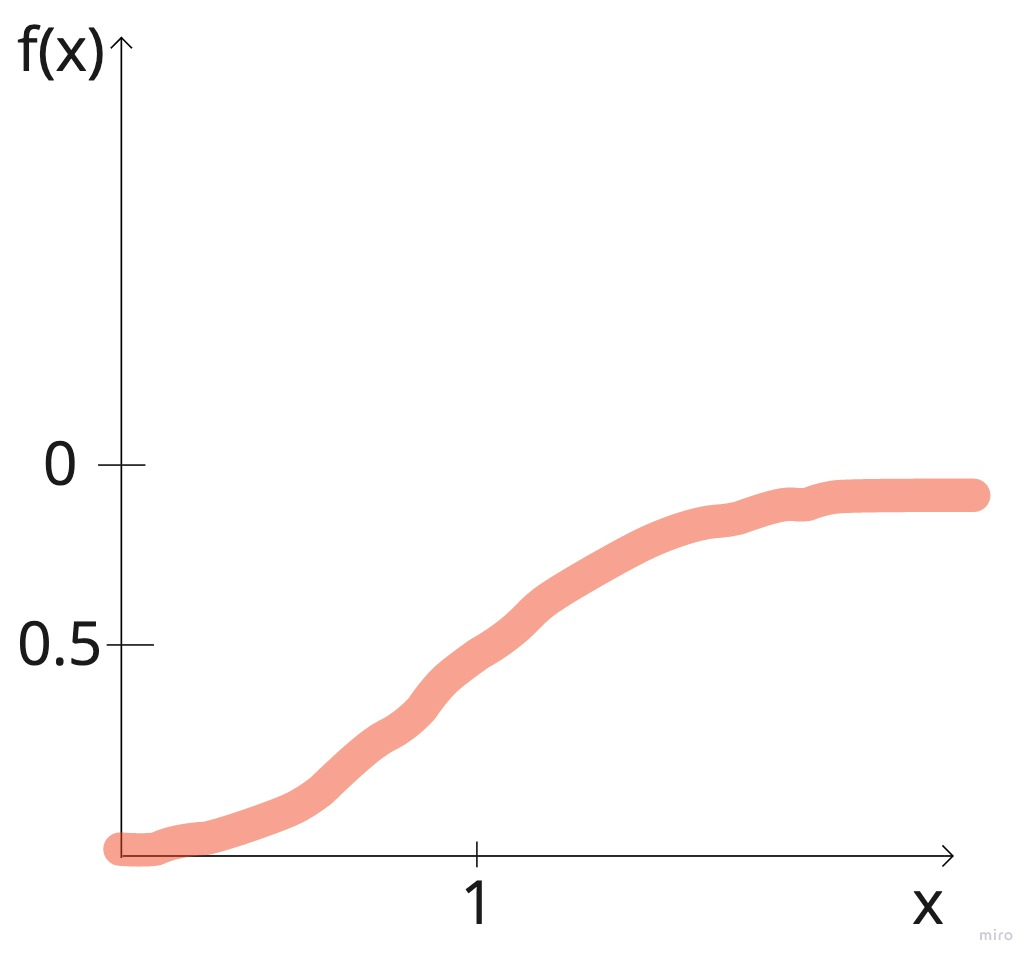
\includegraphics[width=8cm]{images/sigmoid_function.jpg}
    \caption {Sigmoid activation function.}
\end{figure}

\section{From neuron to neural network}
So far we have discussed the properties and functional of a single neuron, which as a result outcomes a linear divide surface in geometrical terms. Meaning when we will concatenate the multiple neurons in some architecture we may achieve some nonlinear divide surfaces.
\begin{figure}[h]
    \centering 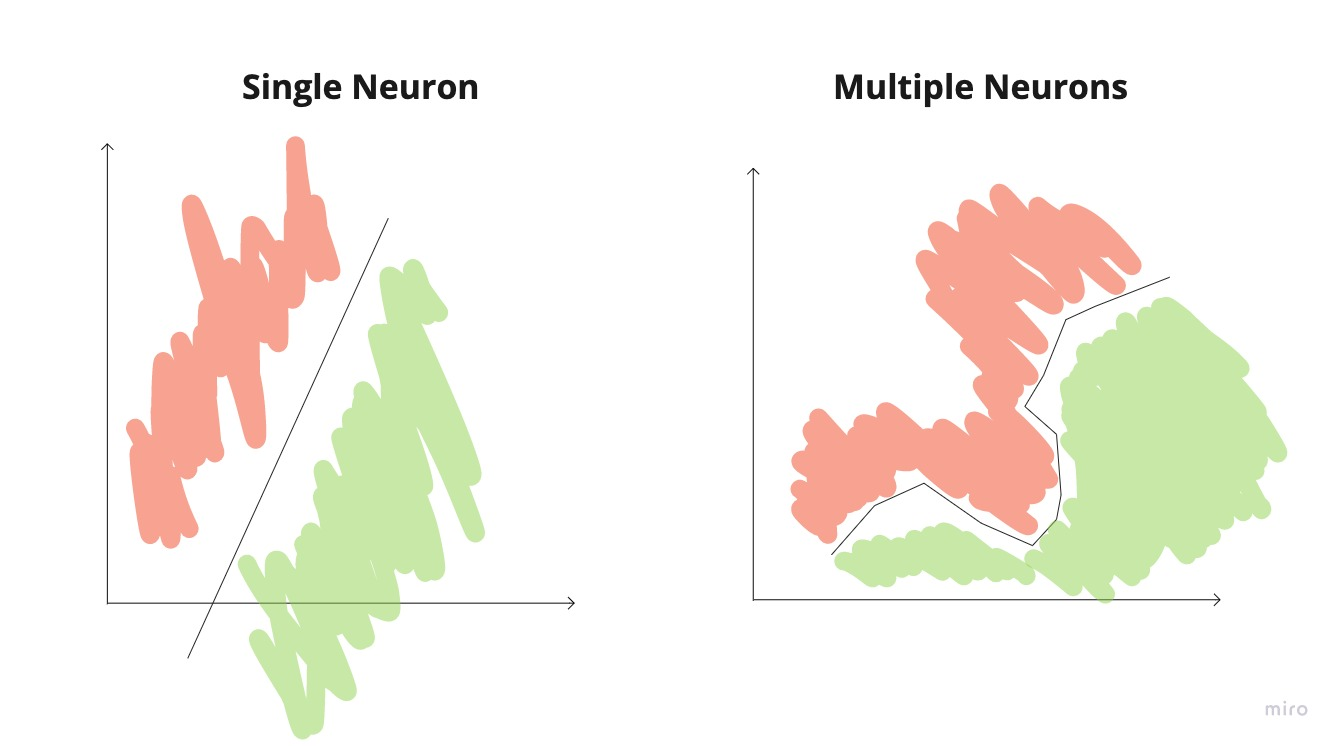
\includegraphics[width=7cm]{images/neuron_to_neural_net.jpg}
    \caption {Sample geometrical representation of dividing surface of step function for single neuron vs multiple neurons.}
\end{figure}

Now the question is how do we get the nonlinear dividing surface. Let us figure it out.
For simplicity define 3 neurons with linear activation function:
\begin{figure}[h]
    \centering 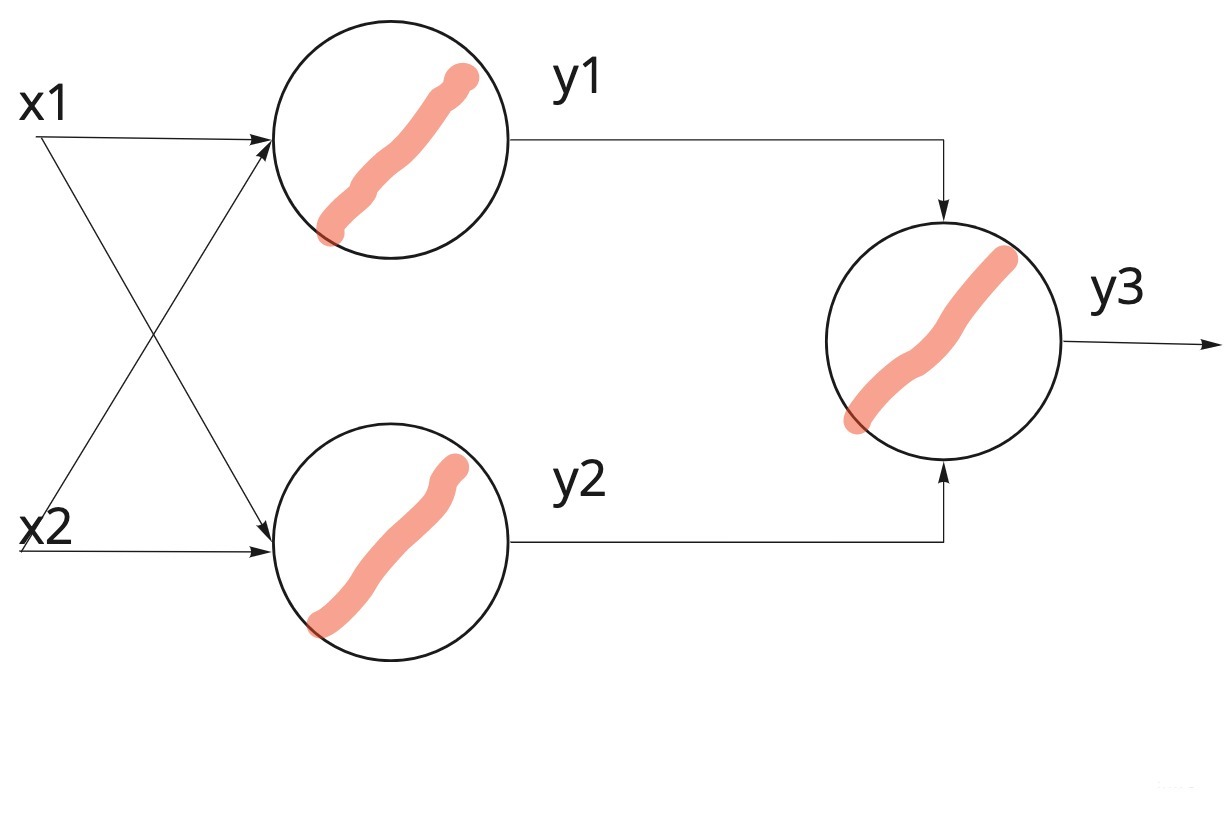
\includegraphics[width=8cm]{images/3_neurons_net.jpg}
    \caption {Sample 1 layer neural net with linear activation functions.}
\end{figure}
The results of performing the net can be considered as:
\[ y_3 = f(w_2^3 \cdot y_2+w_1^3 \cdot y_1+b^3) = \]
By the reason $f$ is simple linear function, equation can be derived as:
\[ = w_2^3 \cdot y_2+w_1^3 \cdot y_1+b^3 = \] 
\[ = w_2^3 \cdot f(w_2^1\cdot x_1+w_2^2 \cdot x_2+b^2) + w_1^3 \cdot f(w_1^1 \cdot x_1+w_1^2 \cdot x_2+b^1) + b^3 = \]   
\[ = w_2^3 \cdot w_2^1 \cdot x_1+w_2^3 \cdot w_2^2 \cdot x_2+b^2 + w_1^3 \cdot w_1^1 \cdot x_1+w_1^3 \cdot w_1^2 \cdot x_2+b^1+b^3 = \]
\[ = x_1[w_2^3 \cdot w_1^2 + w_1^3 \cdot w_1^1] + x_2[w_2^3 \cdot w_2^2 + w_1^3 \cdot w_2^1] + [w_2^3 \cdot b^2+w_1^3 \cdot b^1+b^3] = \]
\[ =  x_1\cdot \tilde{w_1} + x_2\cdot \tilde{w_2} + \tilde{b} \]
Meaning the obtained result is just linear combination of inputs into the neural net. 

\subsection{Neural network starter kit}
Once we had familiarized ourselves with basic concept of neuron and activation function, we may stand a chance to solve some real problem. But still we need figure few more lacking basic components out.
We can be aware of the uniform starter kit for any neural network can be defined as:
\begin{itemize}
    \item neural net architecture, meaning which parts the net will consist of, how the parts will be connected, how neurons will be defined etc.
    \item neural net optimization function, meaning approaching which optimization algorithm the value of loss function (performance of neural net) could be increased. It worth to keep in mind the optimization process requires a loss function to calculate the model error.
    \item neural net loss function, meaning how the net performs. Moreover, the less loss function value is the better performance of the net is.
    \item neural net metrics, meaning how the net performs. It is similar to loss function, but considered as secondary and optional metric. They does not have impact on the neural net fitting process, however could bring out useful insights.    
\end{itemize}


\section{How neural networks learn?}
It was already discussed trivial neural net architecture consisting of neuron mathematically representation and premise of activation function. As for now let us review clause by clause the rest components which are the driven pieces for nets learning process.

\subsection{Optimization function}
Optimization of neural net is the key component in terms of finding latent patterns in input data. The optimization of the net should be considered as the on-the-spot training. There are variety optimization algorithms but the pillar algorithm in the list is gradient descent.
The brief list of optimization algorithms:
\begin{enumerate}
    \item Gradient Descent
    \item Stochastic Gradient Descent
    \item Mini-Batch Gradient Descent
    \item Nesterov Accelerated Gradient
    \item Momentum
    \item Adagrad
    \item RMSProp
\end{enumerate}
Let us discuss how the optimization works under the hood proceeding with the most demonstrative algorithm -- gradient descent.

\subsection{Gradient descent}
Previously we took into consideration the neural net has 2 main tuned parameters: 'weights' and 'bias'.

Let us concern we have a some function which is defined by some levels lines. The function has 2 minimums, which are denoted by the red dots.  It worth to understand by distancing from the minimums the function value increases. 
So far, we have a neural net with some parameters (weights and biases) which performs some value of loss function. As we remember the task is to decrease the value of loss function. Hence, the question is how to do that.

\begin{figure}[h]
    \centering 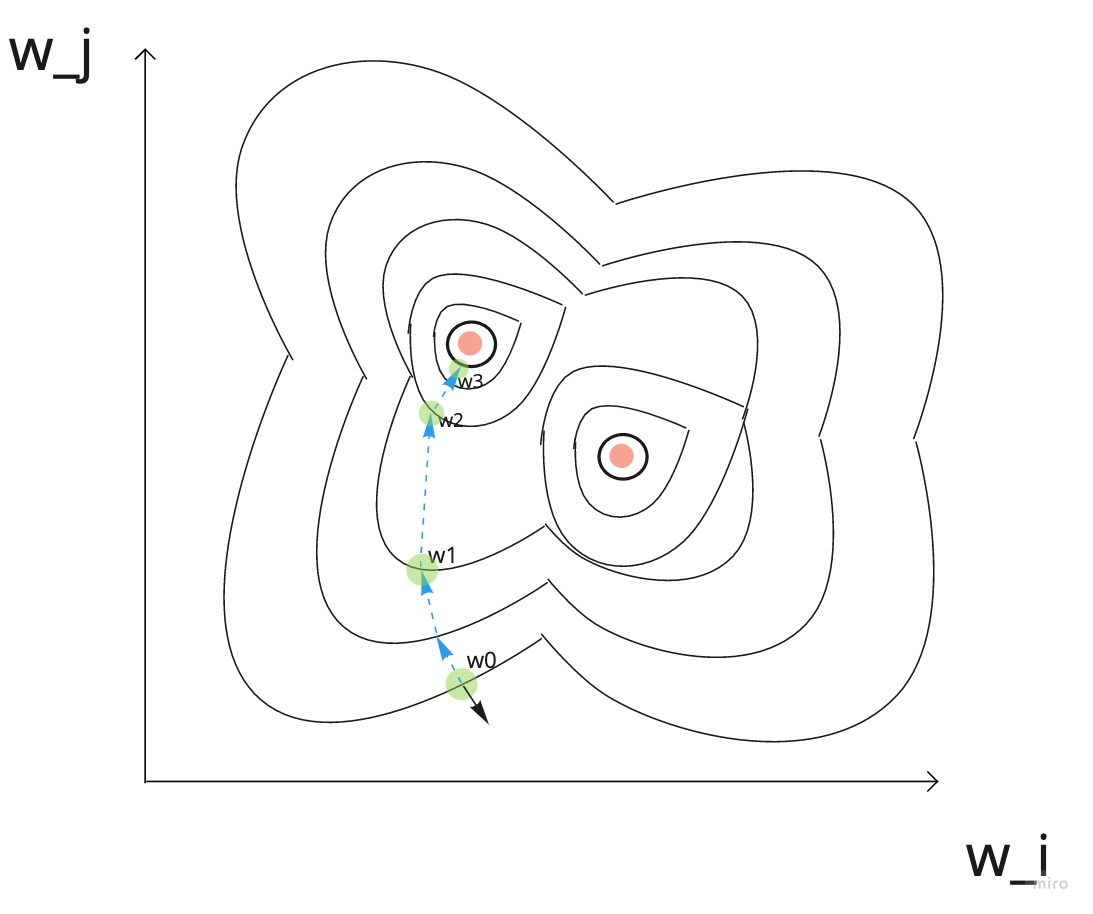
\includegraphics[width=9cm]{images/gradient_descent.jpg}
    \caption {Sample gradient descent visualization.}
\end{figure}

So, the very first provision in the vector of function surface will be defined by $w_0$, where $w_0$ denotes vector of all weights and biases of the net and can be represented as: 

\[ w_0 = [w_1^1, w_1^2,...,w_1^n, w_2^1,...,w_2^n,...,w_n^n, b1^1, b1^2,...,b1^n, b2^1,...,b2^n,...,b_n^n] \]

Accordingly, we need take derivative (meaning gradient, which is vector consisting of derivatives per each coordinate of the function) of the loss function of our vector. It can be represented as:
\[ \delta{f} = [\frac{\partial{f}}{\partial{w_0}}, \frac{\partial{f}}{\partial{w_1}}, ... ,\frac{\partial{f}}{\partial{w_n}} ] \]
As the result, we have calculated the gradient of loss function at the point ($w_0$) where we currently located. The gradient of loss function points out at the direction of greater loss function growth. But, oppositely, we on demand of lower loss function growth, meaning we need to make an opposite step of calculated gradient descent. It can be considered as:
\begin{align*}
w_1 = w_0 - \alpha \cdot \delta{f(w_0)}
\end{align*}
Let us take a closer look at the formula above:
\begin{itemize}
    \item $w_0$: the initial vector of weights and biases of neural net
    \item $\alpha$: parameter for regulating the 'speed' of training the neural net. In other words it affects the size of gradient step 
    \item $\delta{f(w_0)}$: calculated gradient of loss function at the $w_0$ point 
\end{itemize}
The gradient descent of loss function will be calculated until it will not converge some 'preciseness' within predefined 'fallacy'.


\section{How evaluate neural network performance?}
In the terms of an optimization algorithms, function aim to evaluate a distinctive solution (meaning a set of weights) which cite to as objective function. Depending we may search for either to maximize or minimize the objective function. meaning the highest or lowest score respectively.
\subsection{Loss function}
Characteristically neural networks we keen to minimize the error. There are many functions that could be potentially used to estimate error of set of weights in a neural network. Below we consider few popular loss functions.

\subsubsection{Mean Squared Error (MSE)}
Mean Squared Error is the average of the squared error that is used as the loss function for least squares regression. To streamline, MSE is the sum,over all the data points of the square of the difference between the predicted and actual target variables divided by the number of data points.
\begin{align*}
MSE = \frac{{1}}{n} \sum_{i}^{n} (y_i - \widehat{y_i})^2
\end{align*}
where $y$ is the desired Neural Network output, and $\widehat{y_i}$ is the neural network output.

\subsubsection{Cross-Entropy}
Cross-entropy loss, or log loss \footnote{\url{https://ml-cheatsheet.readthedocs.io/en/latest/loss_functions.html#cross-entropy}}, measures the performance of a classification model whose output is a probability value between 0 and 1. Cross-entropy loss increases as the predicted probability diverges from the actual label.
In binary classification, where the number of classes M equals 2 cross-entropy can be calculated as:
\begin{align*}
Cross-Entropy = -{(y\log(p) + (1 - y)\log(1 - p))}
\end{align*}
And if $M > 2$ meaning we work out multi-classification problem we calculate a separate loss for each class label per observation and sum the result as:
\begin{align*}
Cross-Entropy = -\sum_{c=1}^My_{o,c}\log(p_{o,c})
\end{align*}


\section{Convolutional neural networks (CNN)}
What we had discussed before can be considered as usual neural nets in the very general definition. The cons of uniform neural networks are they may perfectly find the latent consistencies however they struggle structured data a lot with. To make it easier to eat up, we should assume the structured data can be representation of the image or bunch of images which refer to some video. Or as well structured data can be representation of the some audio signal.

To highlight the main difference in concepts, let's discuss one example.
Assume there is an RGB image sized $224 \cdot 224$ whereas the dog located in the middle of it. We need to classify whether the dog is on the image. The usual (for instance sigmoid feed forward) neural network will come up with the mask of the dog based on the image. Once new image will be revealed and the dog will not be located in the middle of it, the net will not be able to find and classify the dog. Whilst convolutional neural networks could be generalized independently of the location of the dog, because the convolution itself is invariant operation.         

The neural network architectures which applies convolutions is called convolution neural networks or 'CNN'.    

\subsection{Convolution}
The first layer in CNN is always a convolutional layer. Convolution itself is a mathematical operation on two functions (f and g) that produces a third function $f \cdot g$ that expresses how the shape of one is modified by the other. The convolution in terms of deep learning has following properties:  
\begin{itemize}
    \item number of input channels: number of channels which passes into convolution 
    \item number of output channels: number of output channels of convolution
    \item padding: efficiently adds “space” around input data or feature map – more precisely, “extra rows and columns”. It worth to mention the size of padding always should be $<$ the size of kernel 
    \item kernel (filter) and kernel (filter) size: the filter (matrix) with predefined size and values which is applied step by step (stride) within the data. A very important note is that the depth of filter has to be the same as the depth of the input
    \item stride: consider how the filter 'slides' across the input data
    \item receptive filed: consider the projected area produced by the filter
\end{itemize}

Obtaining of resulting convolution can be described as: as the filter is sliding, or convolving, around the input image, it is multiplying the values in the filter with the original pixel values of the image (aka computing element wise multiplications). These multiplications are all summed up. In mathematical terms the output size of convolution operation is: \[size of output volume = \frac{W-F+2 \cdot P}{S+1} \] where $W$ is the input volume size, $F$ is the receptive field size, $S$ the stride with which they are applied and $P$ is the padding.

How dose convolution work? Assume we have 1 channel image $5 \cdot 5$.
\begin{figure}[h]
    \centering 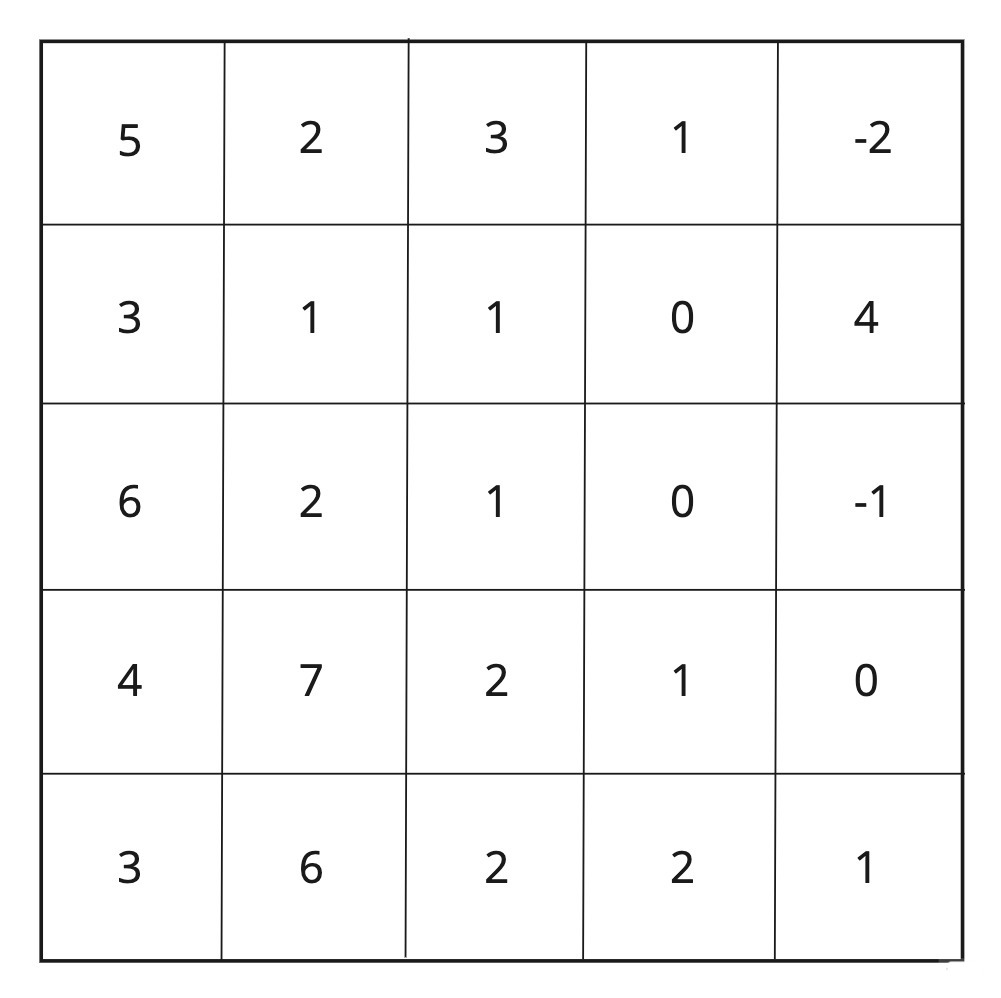
\includegraphics[width=7cm]{images/1_channel.jpg}
    \caption {Sample 1 channel image.}
\end{figure}

We need to calculate the convolution with the filter size $3 \cdot 3$, padding $1 \cdot 1$ and stride $1$. So, let us proceed with the solution. 
\begin{figure}[h]
    \centering 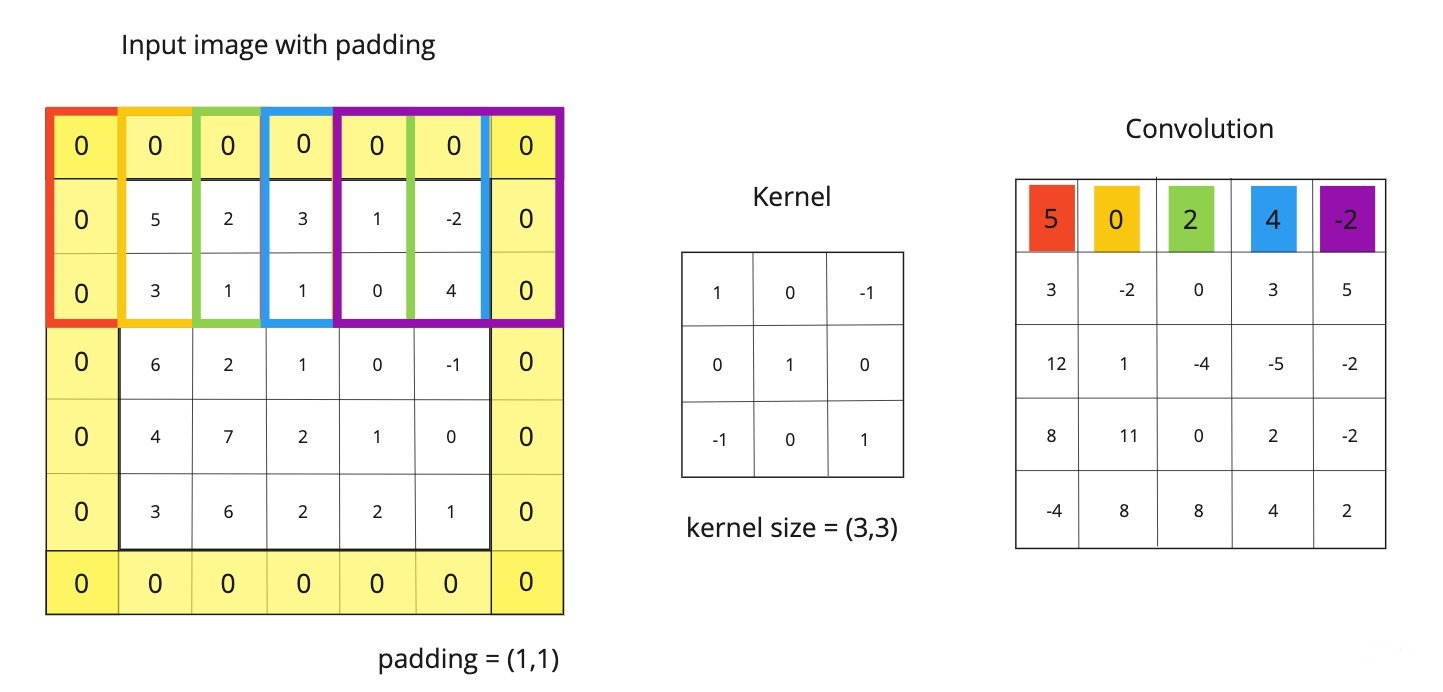
\includegraphics[width=7cm]{images/convolution.jpg}
    \caption {Example of convolution operation.}
\end{figure}

We had defined the filter as: 
\[ \begin{pmatrix} 1 & 0 & -1 \\ 0 & 1 & 0 \\ -1 & 0 & 1 \end{pmatrix} \]

The corresponding calculations are applied clause by clause with step $= 1$, because the stride $= 1$ for all the pixels. Let us take a look at one demonstrative sample:   
\[ \begin{pmatrix} 0 & 0 & 0 \\ 0 & 5 & 2 \\ 0 & 3 & 1 \end{pmatrix} \odot \begin{pmatrix} 1 & 0 & -1 \\ 0 & 1 & 0 \\ -1 & 0 & 1 \end{pmatrix} = \]
\[ = 0 \cdot 1 + 0 \cdot 0 + 0 \cdot (-1) + 0 \cdot 0 + 5 \cdot 1 + 2 \cdot 0 + 0 \cdot (-1) + 3 \cdot 0 + 1 \cdot 1 = \] 
\[ = 0 + 0 + 0 + 0 + 5 + 0 + 0 + 0 + 1= 6 \]
We just have calculated convolution for particular part of the image. 

\subsection{Pooling}
Jointly convolutions it has been frequently applied pooling operation (layer) as well. There is many types of pollings but let us discuss 2 main ones. 

The first pooling type is called max pooling, whereas the second one average pooling. The difference between them obviously is how the calculations are applied. In first case it is taken the maximum value of particular receptive filed, hence in other it is taken the average value of particular receptive filed.

The pooling has 2 properties:
\begin{itemize}
    \item pooling size: consider the size of pooling area 
    \item stride: consider how the pooling 'slides' across the input data 
\end{itemize}    

\begin{figure}[h]
    \centering 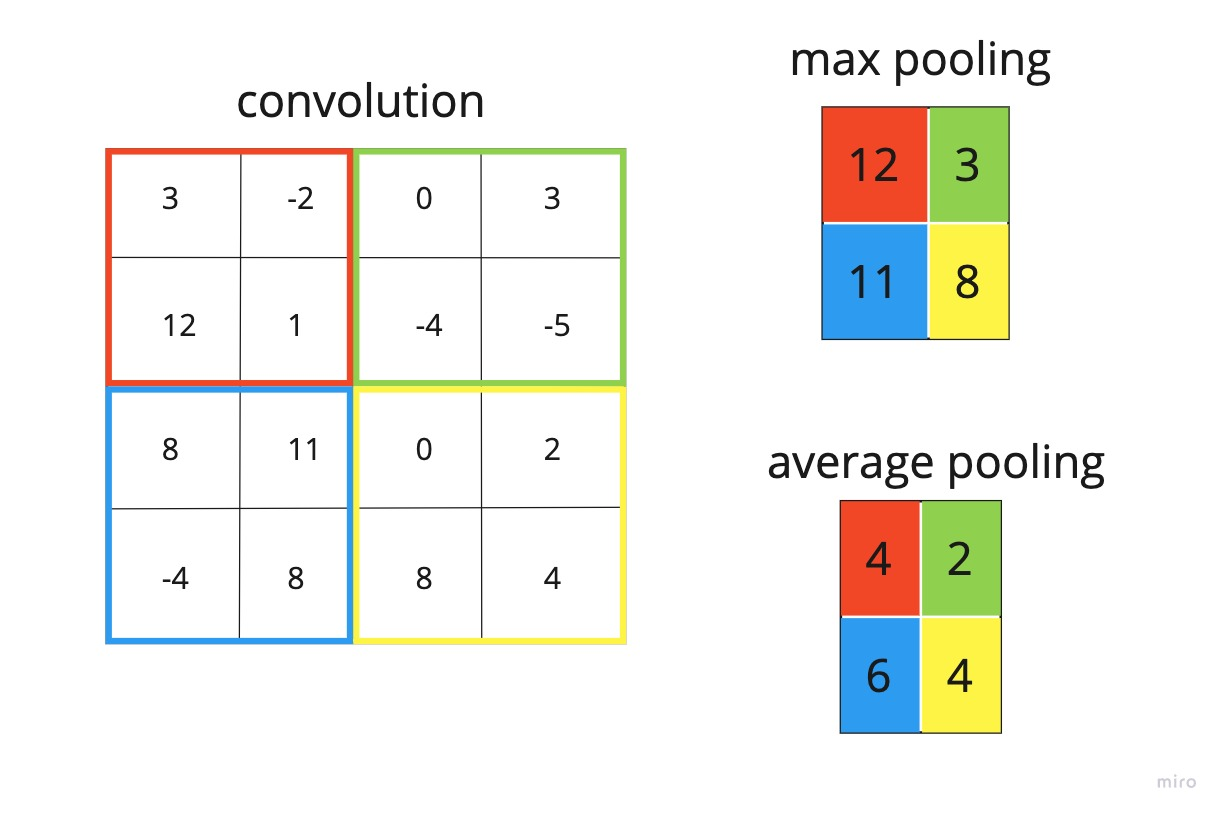
\includegraphics[width=7cm]{images/pooling.jpg}
    \caption {Max pooling versus Average polling.}
\end{figure}

It worth take a look at the example to figure it out. Assume we have some resulting convolution of size $4 \cdot 4$. The pooling layer of size $(2, 2)$ and stride $ = (2, 2)$. 
Applying pooling we have to go through image with stride (2,2) and within corresponding receptive filed calculate either max or average pooling.  

\section{CNN against overfitting}
The overfitting is as important aspect as for instance choosing the proper loss function for particular problem. There are verified means of combating this problem in the context of deep learning. Within below paragraphs we are willing to get to know the various techniques to prevent overfitting of neural networks especially CNN. 

\subsection{Augmentation}
Augmentation itself is not more than applying various image transformations at original image such as cropping, flipping, contrasting, adding and removing noise etc. Afterwards the transformed images are forwarded to the neural network. Literally, it is done by the reason to diversify the data set. Of course exists more advanced techniques based on reinforcement learning, but we will not discuss them within this paper.      

\subsection{Early stopping}
Early stopping is the approach which may stop fitting of the model based on loss function value during validation process. In simplified terms, loss function value can either increase or decrease, whereas we are willing in decreasing of it. Meaning once we detected the increasing of loss, we should stop the learning, because it denotes overfitting.      

\subsection{Regularization}
The purpose of regularization terms is establish additional rules for penalizing the loss function for errors. Meaning the regularization will manage whether the weights are important (good) or not. One of multiple regularization techniques is L2 regularization or so called weight decay. It formed as:
\[ \lambda \cdot \sum_{i=1}^{n} \alpha_i^2 \]

In terms of mean squared error loss function, the addition of regularization considered as:
\[ L = \sum_{i}(\hat{y}-y_i)^2 + \lambda \cdot \sum_{i=1}^{n} \alpha_i^2\]

\subsection{Dropout}
Heretofore, observed regularization terms could be applied both for neural networks and other machine learning architectures. Whilst drop out approach is strictly used for neural nets. There are 2 types of drop out. 

Assume we have 2 layers fully connected neural network, meaning each neuron of first layer is connected with all others of second one. 

As for first type, which is called drop connection. In simplified terms we define the probability $P$ which denotes the probability of dropping of particular connection between particular neurons.  

\begin{figure}[H]
\centering
\begin{minipage}{.48\linewidth}
    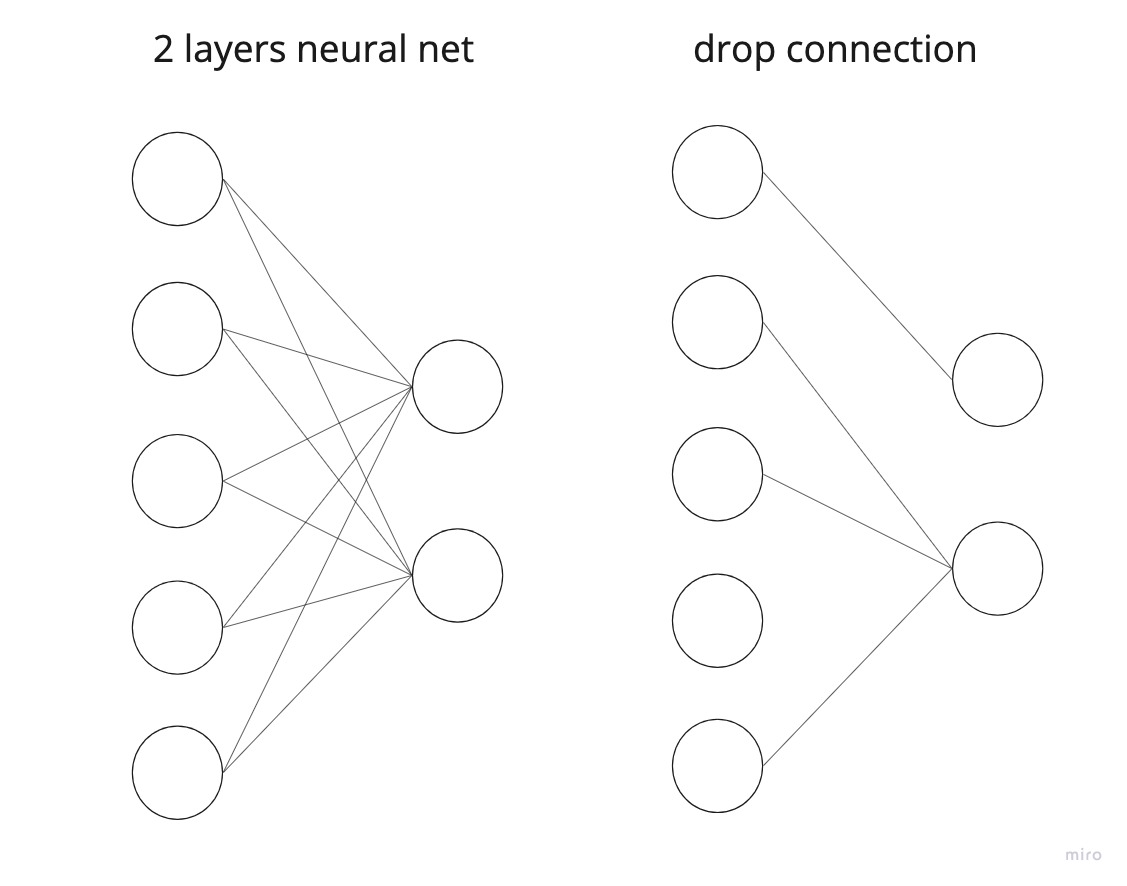
\includegraphics[width=7cm]{images/drop_connection.jpg}
    \caption {Drop connection regularization.}
    \label{fig:drop_connection}
\end{minipage}
\hfill
\begin{minipage}{.48\linewidth}
    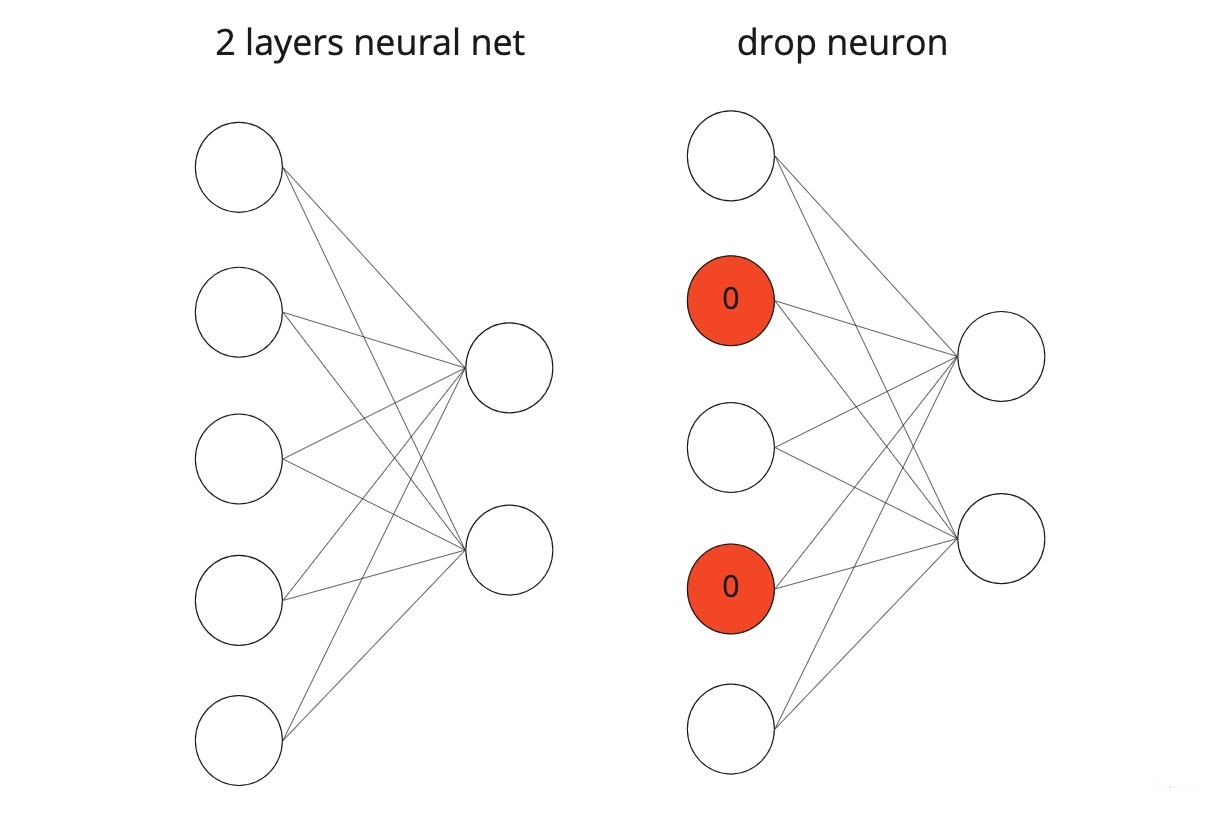
\includegraphics[width=7cm]{images/drop_neuron.jpg}
    \caption {Drop neuron regularization.}
    \label{fig:drop_neuron}
\end{minipage}
\end{figure}

As for second type, which is called drop neuron. In simplified terms we are seeking for neurons which result outputs zero value and then drop it. The corresponding red neurons at \ref{fig:drop_neuron} with value of zero will be removed from the net. We've already get stick with sufficient information to build and derive the particular neural network architecture. 

\section{Unet}
The unet is convolutional network architecture for fast and precise segmentation of images. It was proposed by Olaf Ronneberger, Philipp Fischer, and Thomas Brox at 2015 \cite{Ronneberger2015}. 
\begin{figure}[h]
    \centering 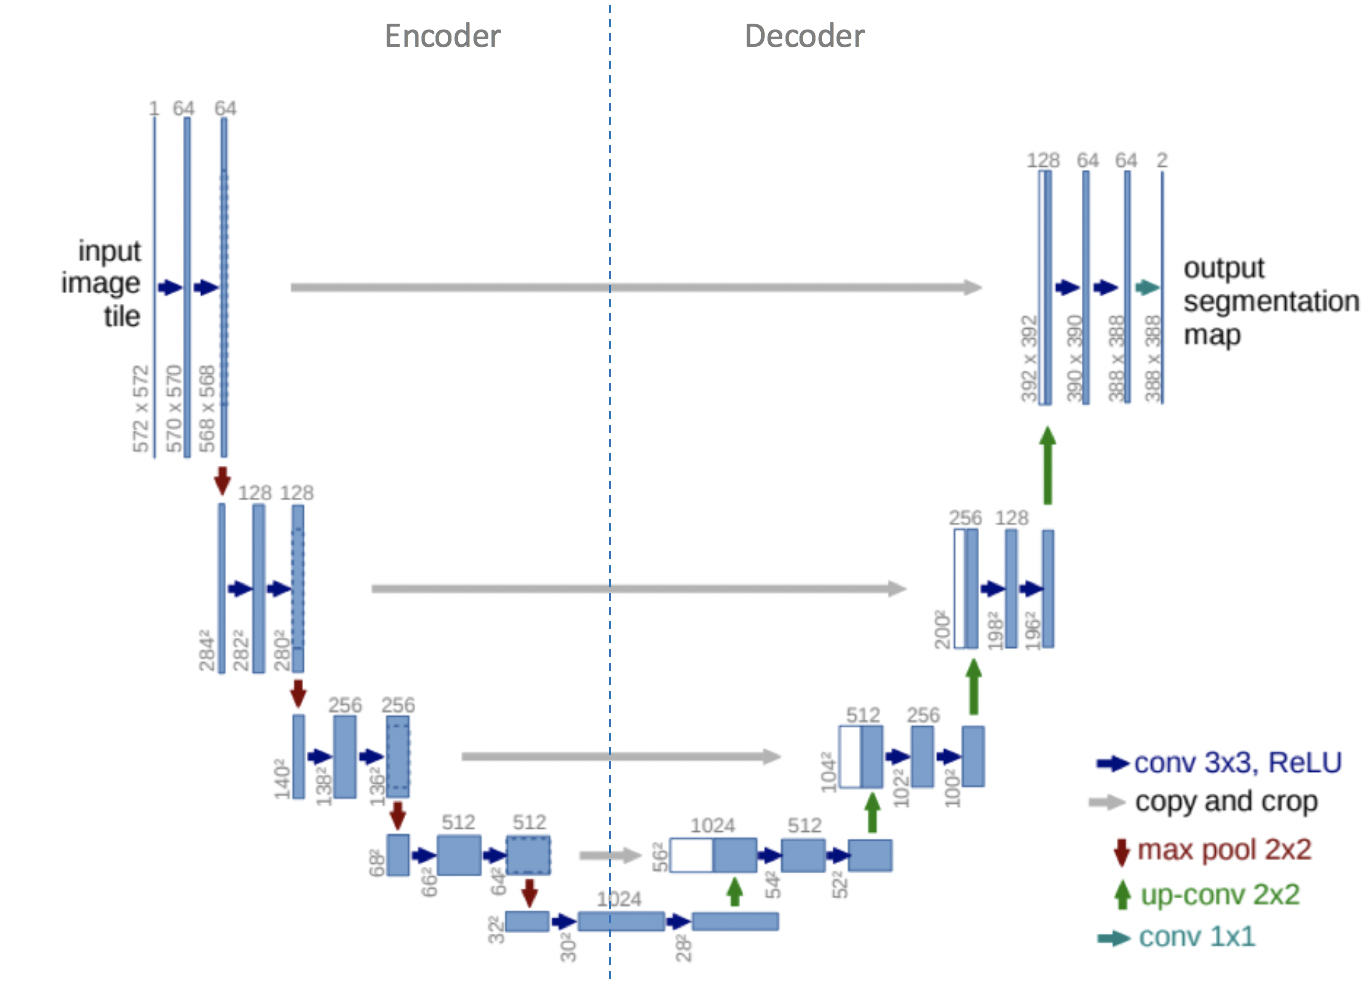
\includegraphics[width=7cm]{images/unet.png}
    \caption {Unet architecture.}
    \small source by: \url{https://arxiv.org/abs/1505.04597}
\end{figure}

Using original terminology of the authors \cite{Ronneberger2015} the net consist of a contracting path (left side) and an expansive path (right side). The contracting path follows the typical architecture of a convolutional network. In simplified terms it can be considered as downsampling or encoder which formed as
a five repeats of double $3 \cdot 3$ convolutions (unpadded convolutions) with rectified linear unit and $2 \cdot 2$ max pooling operation with stride 2. Thus expansive path which can be considered as upsampling or decoder consists of 4 repeats of double $2 \cdot 2$ convolutions (up-convolution) which halve number of feature channels. In total the network has 23 convolutional layers. The architecture implementation can be find within bare unet github gist \footnote { \url{https://gist.github.com/f8eb74d57b914878d52c47ac359758e8.git}}

